\section{MOSFET}

\subsection{Structure}

\begin{wrapfigure}{r}{0.5\textwidth}
    \centering
    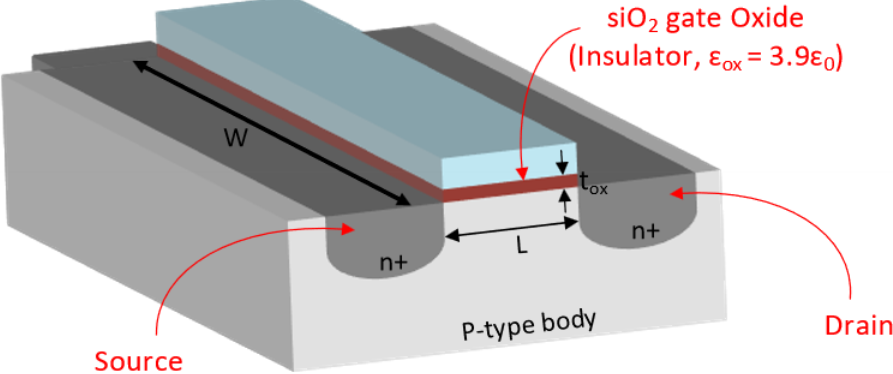
\includegraphics[scale=0.5]{images/MOSFET.png}
    \caption{MOSFET}
\end{wrapfigure}

The given image shows a MOSFET with P-type boday and N-type source and drain. This is a NMOS transistor. Voltage applied to gate will allow current to flow from source to drain.

\begin{itemize}
    \item \textbf{Polysilicon}: Silicon formed from many small silicon crystals.
    \item \textbf{Gate Oxide}: Insulating layer between the gate and the channel.
    \item Source and Drain are doped with N-type impurities. PMOS has P-type impurities with body as N-type.
    \item \textbf{Bulk}: Body of the transistor.
\end{itemize}

\subsection{NMOS and PMOS}

Drain-Source current is controlled by the gate-source voltage.

\begin{wrapfigure}{l}{1\textwidth}
    \centering
    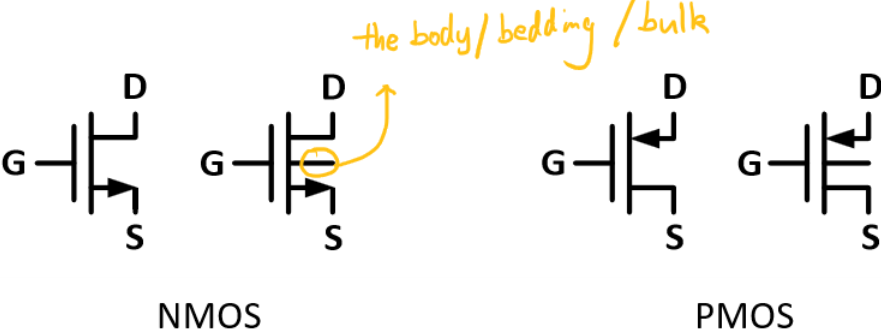
\includegraphics[scale=0.5]{images/NMOSandPMOS.png}
    \caption{MOSFET}
\end{wrapfigure}

\begin{itemize}
    \item \textbf{NMOS}: When $V_{GS} > V_{th}$, the transistor is on. When $V_{GS} < V_{th}$, the transistor is off.
    \item \textbf{PMOS}: When $V_{GS} < V_{th}$, the transistor is on. When $V_{GS} > V_{th}$, the transistor is off.
\end{itemize}